\PassOptionsToPackage{dvipsnames,svgnames,x11names}{xcolor}
\documentclass[tikz,border=8pt]{standalone}
\usetikzlibrary{arrows.meta,positioning,calc,shapes,shadows,decorations.pathmorphing,shapes.geometric,backgrounds,decorations.markings,decorations.pathreplacing,decorations.text,fit,shapes.misc,shapes.arrows,matrix,bending,3d,chains,intersections,shapes.symbols,svg.path,shapes.multipart,snakes,shapes.callouts,angles,quotes}
\providecolor{gold}{RGB}{212,175,55}
\providecolor{silver}{RGB}{192,192,192}
\providecolor{bronze}{RGB}{205,127,50}
\providecolor{darkblue}{RGB}{0,0,139}
\providecolor{lightblue}{RGB}{173,216,230}
\providecolor{darkgreen}{RGB}{0,100,0}
\providecolor{lightgreen}{RGB}{144,238,144}
\providecolor{darkred}{RGB}{139,0,0}
\providecolor{navy}{RGB}{0,0,128}
\providecolor{skyblue}{RGB}{135,206,235}
\providecolor{beige}{RGB}{245,245,220}
\providecolor{cream}{RGB}{255,253,208}
\usepackage{amsmath}
\usepackage{amssymb}
\usepackage{fontawesome5}
\usetikzlibrary{fadings,shadows.blur,patterns,patterns.meta}

\providecolor{gold}{RGB}{212,175,55}
\providecolor{silver}{RGB}{192,192,192}
\providecolor{bronze}{RGB}{205,127,50}
\providecolor{darkblue}{RGB}{0,0,139}
\providecolor{lightblue}{RGB}{173,216,230}
\providecolor{darkgreen}{RGB}{0,100,0}
\providecolor{lightgreen}{RGB}{144,238,144}
\providecolor{darkred}{RGB}{139,0,0}
\providecolor{navy}{RGB}{0,0,128}
\providecolor{skyblue}{RGB}{135,206,235}
\providecolor{beige}{RGB}{245,245,220}
\providecolor{cream}{RGB}{255,253,208}
\usepackage{amsmath}
\usepackage{amssymb}
\usepackage{fontawesome5}

\usepackage{xcolor}
\usepackage{tikz}

% --- COLOR PALETTE DEFINITION ---
\definecolor{headerCol}{RGB}{31, 41, 55}       % #1F2937 Deep Slate
\definecolor{textMuted}{RGB}{75, 85, 99}        % #4B5563 Muted Text
\definecolor{panelBg}{RGB}{249, 250, 251}       % #F9FAFB Off-White
\definecolor{panelBorder}{RGB}{229, 231, 235}   % #E5E7EB Light Gray Border

\definecolor{mediaCol}{RGB}{109, 40, 217}       % #6D28D9 Deep Violet
\definecolor{mediaFill}{RGB}{237, 233, 254}     % #EDE9FE Soft Violet
\definecolor{mediaDark}{RGB}{91, 33, 182}       % #5B21B6 Violet Dark

\definecolor{cntCol}{RGB}{5, 150, 105}          % #059669 Emerald Green Accent
\definecolor{cntBorder}{RGB}{52, 211, 153}      % #34D399 Emerald Border
\definecolor{cntFill}{RGB}{240, 253, 244}       % #F0FDF4 Soft Emerald

\definecolor{voidCol}{RGB}{225, 29, 72}         % #E11D48 Rose Red
\definecolor{voidFill}{RGB}{255, 228, 230}      % #FFE4E6 Soft Rose
\definecolor{voidBorder}{RGB}{251, 113, 133}    % #FB7185 Rose Border

\definecolor{macRed}{RGB}{239, 68, 68}
\definecolor{macYellow}{RGB}{245, 158, 11}
\definecolor{macGreen}{RGB}{16, 185, 129}

\begin{document}
\begin{tikzpicture}[
    show background rectangle,
    background rectangle/.style={fill=white},
    every node/.style={font=\sffamily, text=headerCol},
    panel/.style={fill=panelBg, draw=panelBorder, line width=1.2pt, rounded corners=8pt, blur shadow={shadow opacity=18, shadow yshift=-3pt, shadow blur radius=6pt}},
    pill/.style={font=\bfseries\small, text=white, rounded corners=4pt, inner sep=6pt, blur shadow={shadow opacity=15, shadow yshift=-1.5pt}},
    mathBox/.style={fill=white, draw=mediaCol!30, line width=0.8pt, rounded corners=5pt, inner sep=6pt, font=\small, align=center, blur shadow={shadow opacity=10, shadow yshift=-1pt}}
]

% ==========================================
% 1. GLOBAL HEADER & TITLES (CENTER X = 0)
% ==========================================
\node[font=\Huge\bfseries, text=headerCol] at (0.0547,16.601) {Aspect Ratio Inversion \& Bounding Voids};
\node[font=\Large, text=textMuted] at (0.0547,15.601) {Geometric derivations of Letterboxing and Pillarboxing in \texttt{object-fit: contain}};

% Central Divergence Node & Layered Arrows
\node[draw=headerCol!35, fill=white, line width=1.1pt, rounded corners=6pt, font=\bfseries\small, text=headerCol, inner sep=6pt, blur shadow={shadow opacity=18, shadow yshift=-2pt, shadow blur radius=4pt}] (div) at (0, 6.2) {$\min(S_x, S_y)$ Divergence};

\draw[-Latex=3mm, line width=3.5pt, mediaCol!25] (div.west) -- (-3, 6.2);
\draw[-Latex=3mm, line width=1.5pt, mediaCol] (div.west) -- (-3, 6.2);

\draw[-Latex=3mm, line width=3.5pt, mediaCol!25] (div.east) -- (3, 6.2);
\draw[-Latex=3mm, line width=1.5pt, mediaCol] (div.east) -- (3, 6.2);


% ==========================================
% 2. SCENARIO A: LETTERBOXING (LEFT PANEL, CENTER X = -8)
% ==========================================
% A. Structural Background
\draw[panel] (-13.0, -3.5) rectangle (-3.0, 14.5);
\node[pill, fill=headerCol] at (-8, 13.5) {\faFilm\ \ SCENARIO A: $R_{src} > R_{cnt}$};

% B. Source Media Box (16:9 Landscape, Center: (-8, 10.5))
\draw[draw=mediaCol, fill=mediaFill!45, line width=1.2pt, rounded corners=6pt, blur shadow={shadow opacity=12, shadow yshift=-2pt}] (-10.4, 9.15) rectangle (-5.6, 11.85);

% UI Top Control Bar (macOS style)
\fill[mediaCol!15, rounded corners=5pt] (-10.38, 11.45) rectangle (-5.62, 11.83);
\fill[mediaCol!15] (-10.38, 11.45) rectangle (-5.62, 11.60);
\fill[macRed] (-10.1, 11.64) circle (0.07);
\fill[macYellow] (-9.85, 11.64) circle (0.07);
\fill[macGreen] (-9.6, 11.64) circle (0.07);

% Wireframe Media Icon (Mountain & Sun) relative to (-8, 10.5)
\draw[mediaCol!35, fill=mediaCol!20] (-7.3, 10.3) circle (0.22);
\draw[mediaCol!40, fill=mediaCol!15, line join=round] (-9.0, 9.3) -- (-8.2, 9.9) -- (-7.6, 9.5) -- (-6.8, 9.8) -- (-6.5, 9.5) -- (-6.5, 9.3) -- cycle;
\node[font=\bfseries, text=mediaCol] at (-8, 10.9) {Landscape Media (16:9)};

% Dimension Brackets for Media Box
\draw[decorate, decoration={brace, amplitude=4pt, raise=4pt}, textMuted, semithick] (-10.4, 12.0) -- (-5.6, 12.0) node[midway, above=4pt, font=\scriptsize\bfseries] {$W_{src} = 16$};
\draw[decorate, decoration={brace, amplitude=4pt, raise=4pt}, textMuted, semithick] (-5.4, 11.85) -- (-5.4, 9.15) node[midway, right=4pt, font=\scriptsize\bfseries] {$H_{src} = 9$};

% C. Informational Block
\node[text width=8.5cm, align=center] at (-8, 7.8) {
    Media Aspect Ratio is \textbf{greater} than the Container.\\
    \textbf{Mathematical Output:} Width dictates the scale factor limit.
};

\node[mathBox] at (-8, 6.2) {
    $S_x = \dfrac{W_{cnt}}{W_{src}} = \dfrac{4}{16} = 0.25, \quad S_y = \dfrac{H_{cnt}}{H_{src}} = \dfrac{5}{9} \approx 0.556$\\[4pt]
    $\implies S = \min(S_x, S_y) = S_x$
};

% D. The Rendering Engine (DOM Container 4:5)
\node[font=\small\bfseries, text=cntCol, fill=white, draw=cntBorder, rounded corners=4pt, inner sep=3pt, blur shadow={shadow opacity=10, shadow yshift=-1pt}] at (-8.018,4.8899) {Portrait DOM Container (4:5)};
\draw[very thick, cntBorder, dashed, fill=cntFill!35, rounded corners=6pt] (-10, -0.7) rectangle (-6, 4.3);

% Dimensions
\draw[decorate, decoration={brace, amplitude=4pt, mirror, raise=10pt}, cntCol!80, semithick] (-10.2, 4.3) -- (-10.2, -0.7) node[midway, left=5pt, font=\scriptsize\bfseries] {$H_{cnt} = 5$};
\draw[decorate, decoration={brace, amplitude=4pt, mirror, raise=3pt}, cntCol!80, semithick] (-10, -0.8) -- (-6, -0.8) node[midway, below=5pt, font=\scriptsize\bfseries] {$W_{cnt} = 4$};

% Top Void (Letterbox)
\fill[voidFill!80, draw=voidBorder, thick, rounded corners=2pt] (-10, 2.925) rectangle (-6, 4.3);
\fill[pattern=north west lines, pattern color=voidCol!35, rounded corners=2pt] (-10, 2.925) rectangle (-6, 4.3);
\node[font=\small\bfseries, text=voidCol, fill=voidFill!90, inner sep=2pt, rounded corners=2pt] at (-8.0, 3.6125) {Letterbox Void (Top)};

% Bottom Void (Letterbox)
\fill[voidFill!80, draw=voidBorder, thick, rounded corners=2pt] (-10, -0.7) rectangle (-6, 0.675);
\fill[pattern=north west lines, pattern color=voidCol!35, rounded corners=2pt] (-10, -0.7) rectangle (-6, 0.675);
\node[font=\small\bfseries, text=voidCol, fill=voidFill!90, inner sep=2pt, rounded corners=2pt] at (-8.0, -0.0125) {Letterbox Void (Bottom)};

% Scaled Matrix (The Result)
\fill[mediaCol!85, draw=mediaDark, thick, rounded corners=3pt, blur shadow={shadow opacity=20, shadow yshift=-1.5pt}] (-10, 0.675) rectangle (-6, 2.925);
\begin{scope}[shift={(-8, 1.8)}, scale=0.8333]
    \draw[white!40, fill=white!20] (0.7, -0.1) circle (0.22);
    \draw[white!50, fill=white!25, line join=round] (-1.2, -1.0) -- (-0.4, -0.3) -- (0.1, -0.7) -- (0.8, -0.4) -- (1.2, -0.8) -- (1.2, -1.0) -- cycle;
\end{scope}
\node[font=\bfseries, text=white, align=center] at (-8, 2.5) {Scaled Matrix};

% Boundary Touch Indicators (Limit Reached on X-Axis)
\draw[orange, line width=2.5pt] (-10, 0.675) -- (-10, 2.925);
\draw[orange, line width=2.5pt] (-6, 0.675) -- (-6, 2.925);

\draw[-Latex, thick, orange!90!black] (-12.4, 2.7) -- (-10.1, 2.7) node[pos=0, left, font=\scriptsize\bfseries, text width=1.6cm, align=right] {X-Axis Limit Reached};
\draw[-Latex, thick, orange!90!black] (-3.6, 2.7) -- (-5.9, 2.7) node[pos=0, right, font=\scriptsize\bfseries, text width=1.6cm, align=left] {X-Axis Limit Reached};

% E. Narrative Footer
\node[anchor=north, text width=8.8cm, align=justify, font=\small, text=headerCol!85] at (-8.0, -1.5) {
    The horizontal X-axis hits the container bounds first. To strictly maintain the 16:9 pixel aspect ratio, Y-axis interpolation stops early, leaving geometric voids above and below.
};


% ==========================================
% 3. SCENARIO B: PILLARBOXING (RIGHT PANEL, CENTER X = 8)
% ==========================================
% A. Structural Background
\draw[panel] (3.0539,-4.129) rectangle (13.0, 14.5);
\node[pill, fill=headerCol] at (8.0547,13.992) {\faIcon{mobile-alt}\ \ SCENARIO B: $R_{src} < R_{cnt}$};

% B. Source Media Box (9:16 Portrait, Center: (8, 10.5))
\draw[draw=mediaCol, fill=mediaFill!45, line width=1.2pt, rounded corners=6pt, blur shadow={shadow opacity=12, shadow yshift=-2pt}] (6.875, 8.5) rectangle (9.125, 12.5);

% UI Top Notch (Mobile style)
\fill[mediaCol!15, rounded corners=5pt] (6.895, 12.1) rectangle (9.105, 12.48);
\fill[mediaCol!15] (6.895, 12.1) rectangle (9.105, 12.25);
\fill[mediaCol!40, rounded corners=1.5pt] (7.75, 12.24) rectangle (8.25, 12.36);

% Wireframe Media Icon relative to (8, 10.5)
\draw[mediaCol!35, fill=mediaCol!20] (8.5, 9.8) circle (0.16);
\draw[mediaCol!40, fill=mediaCol!15, line join=round] (7.2, 8.8) -- (7.6, 9.4) -- (8.0, 9.0) -- (8.5, 9.3) -- (8.8, 9.0) -- (8.8, 8.8) -- cycle;
\node[font=\bfseries, text=mediaCol, align=center] at (8, 11.3) {Portrait\\(9:16)};

% Dimension Brackets for Media Box
\draw[decorate, decoration={brace, amplitude=4pt, raise=4pt}, textMuted, semithick] (6.875, 12.7) -- (9.125, 12.7) node[midway, above=4pt, font=\scriptsize\bfseries] {$W_{src} = 9$};
\draw[decorate, decoration={brace, amplitude=4pt, raise=4pt}, textMuted, semithick] (9.225, 12.5) -- (9.225, 8.5) node[midway, right=4pt, font=\scriptsize\bfseries] {$H_{src} = 16$};

% C. Informational Block
\node[text width=8.5cm, align=center] at (8, 7.8) {
    Media Aspect Ratio is \textbf{less} than the Container.\\
    \textbf{Mathematical Output:} Height dictates the scale factor limit.
};

\node[mathBox] at (8, 6.2) {
    $S_x = \dfrac{W_{cnt}}{W_{src}} = \dfrac{16}{9} \approx 1.778, \quad S_y = \dfrac{H_{cnt}}{H_{src}} = \dfrac{9}{16} \approx 0.563$\\[4pt]
    $\implies S = \min(S_x, S_y) = S_y$
};

% D. The Rendering Engine (DOM Container 16:9)
\node[font=\small\bfseries, text=cntCol, fill=white, draw=cntBorder, rounded corners=4pt, inner sep=3pt, blur shadow={shadow opacity=10, shadow yshift=-1pt}] at (7.8561,5.0336) {Landscape DOM Container (16:9)};
\draw[very thick, cntBorder, dashed, fill=cntFill!35, rounded corners=6pt] (5.333, 0.3) rectangle (10.666, 3.3);

% Dimensions
\draw[decorate, decoration={brace, amplitude=4pt, raise=3pt}, cntCol!80, semithick] (10.766, 3.3) -- (10.766, 0.3) node[midway, right=5pt, font=\scriptsize\bfseries] {$H_{cnt} = 9$};
\draw[decorate, decoration={brace, amplitude=4pt, mirror, raise=3pt}, cntCol!80, semithick] (5.333,-0.4046) -- (10.666,-0.4046) node[midway, below=5pt, font=\scriptsize\bfseries] {$W_{cnt} = 16$};

% Left Void (Pillarbox)
\fill[voidFill!80, draw=voidBorder, thick, rounded corners=2pt] (5.333, 0.3) rectangle (7.156, 3.3);
\fill[pattern=north west lines, pattern color=voidCol!35, rounded corners=2pt] (5.333, 0.3) rectangle (7.156, 3.3);
\node[font=\footnotesize\bfseries, text=voidCol, fill=voidFill!90, inner sep=2pt, rounded corners=2pt, align=center, text width=1.5cm] at (6.244, 1.8) {Pillarbox\\(Left)};

% Right Void (Pillarbox)
\fill[voidFill!80, draw=voidBorder, thick, rounded corners=2pt] (8.844, 0.3) rectangle (10.666, 3.3);
\fill[pattern=north west lines, pattern color=voidCol!35, rounded corners=2pt] (8.844, 0.3) rectangle (10.666, 3.3);
\node[font=\footnotesize\bfseries, text=voidCol, fill=voidFill!90, inner sep=2pt, rounded corners=2pt, align=center, text width=1.5cm] at (9.755, 1.8) {Pillarbox\\(Right)};

% Scaled Matrix (The Result)
\fill[mediaCol!85, draw=mediaDark, thick, rounded corners=3pt, blur shadow={shadow opacity=20, shadow yshift=-1.5pt}] (7.156, 0.3) rectangle (8.844, 3.3);
\begin{scope}[shift={(8, 1.8)}, scale=0.75]
    \draw[white!40, fill=white!20] (0.5, 0.2) circle (0.16);
    \draw[white!50, fill=white!25, line join=round] (-0.8, -1.0) -- (-0.3, -0.4) -- (0.1, -0.8) -- (0.6, -0.5) -- (0.9, -0.8) -- (0.9, -1.0) -- cycle;
\end{scope}
\node[font=\bfseries, text=white, align=center] at (8, 2.7) {Scaled\\Matrix};

% Boundary Touch Indicators (Limit Reached on Y-Axis)
\draw[orange, line width=2.5pt] (7.156, 3.3) -- (8.844, 3.3);
\draw[orange, line width=2.5pt] (7.156, 0.3) -- (8.844, 0.3);

\draw[-Latex, thick, orange!90!black] (8,4.3046) -- (8.0, 3.4) node[pos=0, above, font=\scriptsize\bfseries, align=center] {Y-Axis Limit Reached};
\draw[-Latex, thick, orange!90!black] (8,-0.8046) -- (8.0, 0.2) node[pos=0, below, font=\scriptsize\bfseries, align=center] {Y-Axis Limit Reached};

% E. Narrative Footer
\node[anchor=north, text width=8.8cm, align=justify, font=\small, text=headerCol!85] at (8.0539,-2.129) {
    The vertical Y-axis hits the container bounds first. To strictly maintain the 9:16 pixel aspect ratio, X-axis interpolation stops early, generating geometric voids on the horizontal flanks.
};

\end{tikzpicture}
\end{document}
